\vspace{-0.05in}
\section{Influence Probability Estimation Model}
\label{sec:influenceprob}

\begin{figure*}
\centering
\subfloat[]{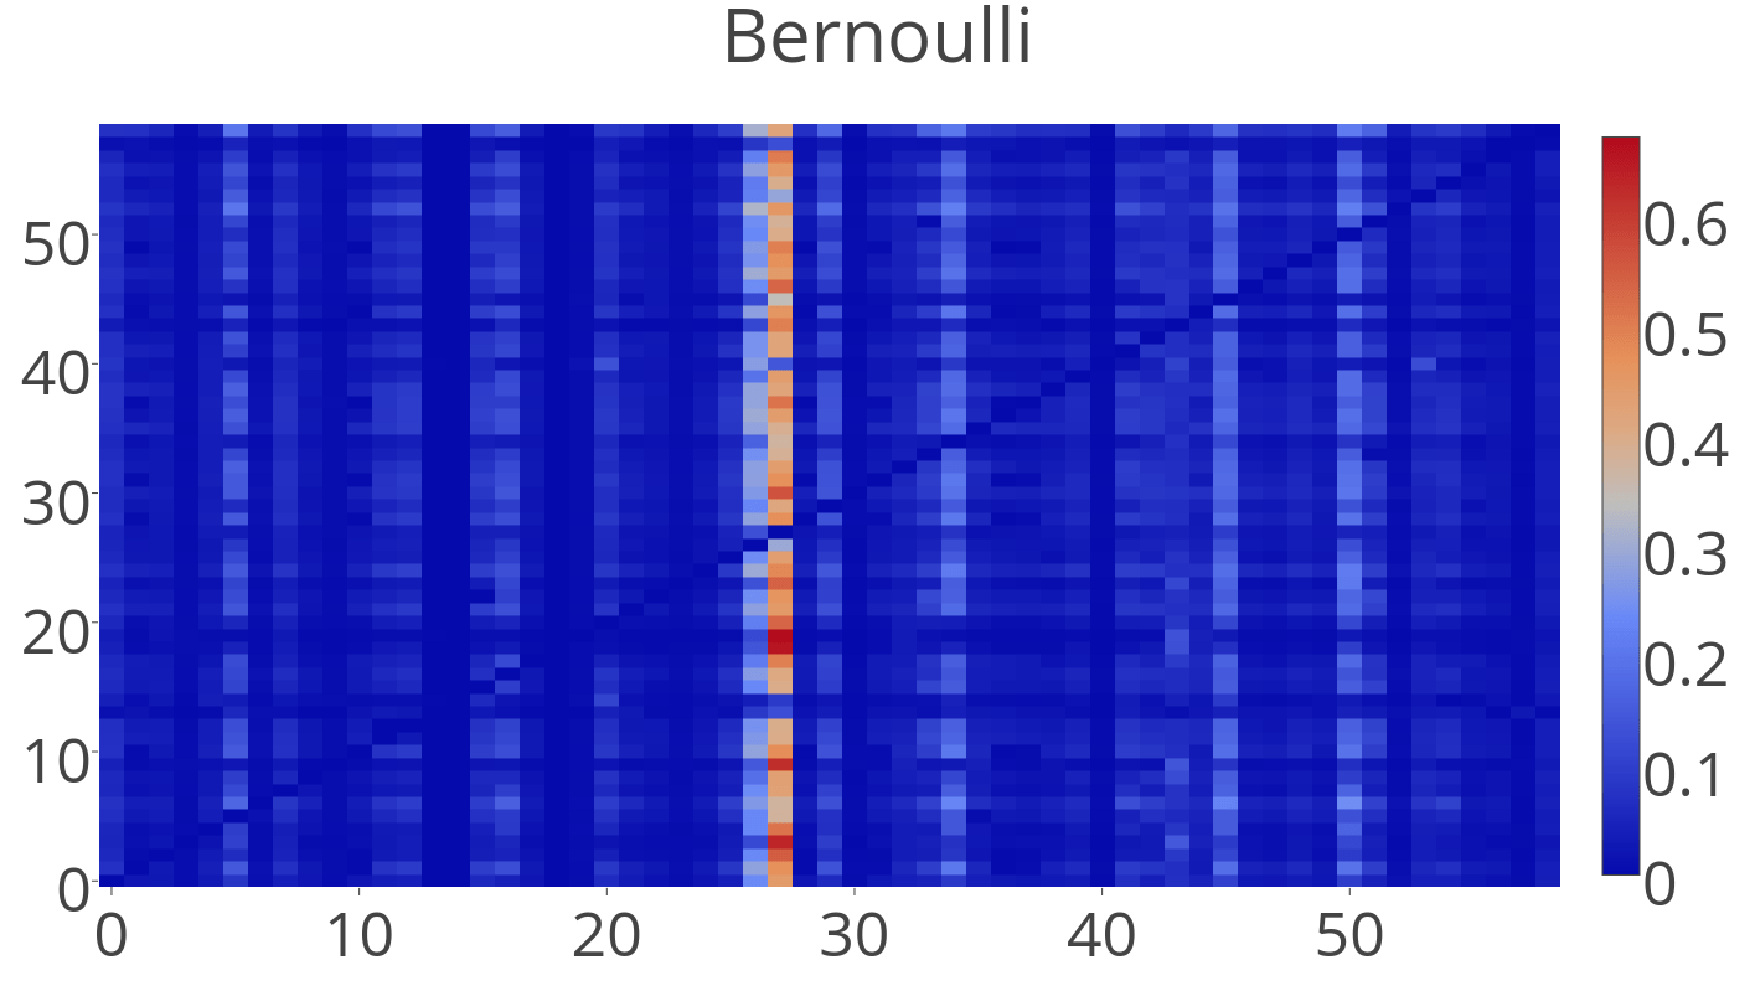
\includegraphics[width=0.24\linewidth]{figure/bernoulli-train}\label{fig:moredata1}} 
\subfloat[]{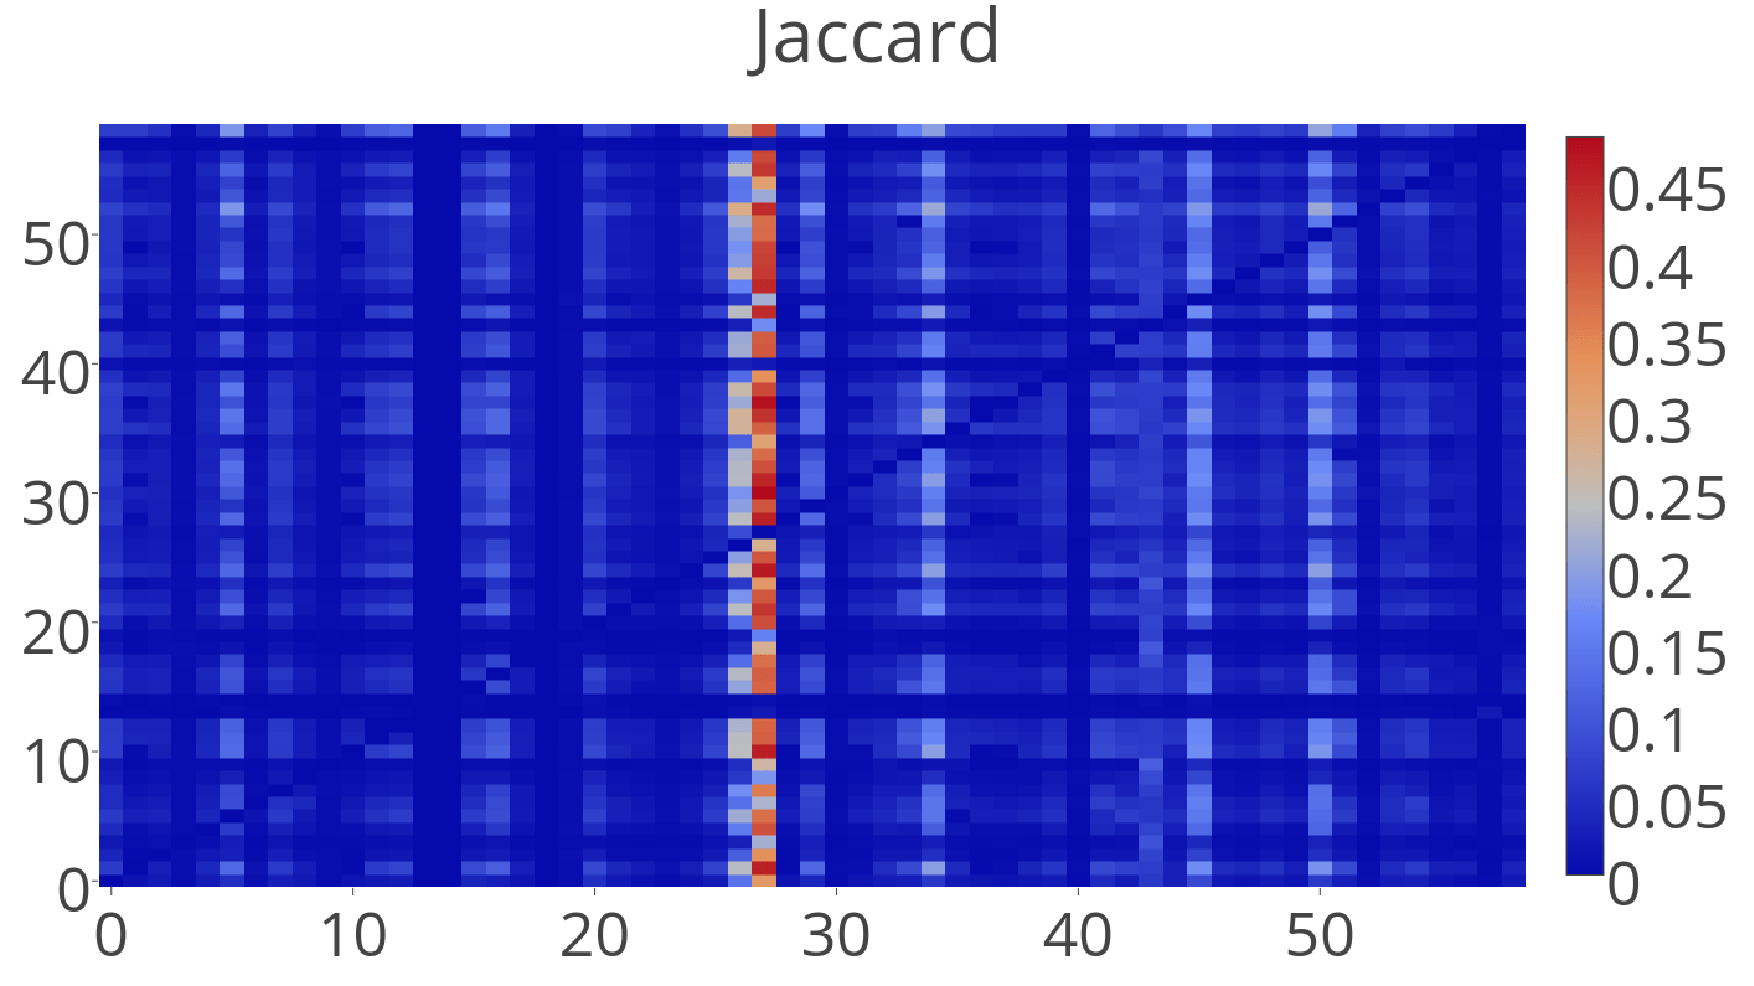
\includegraphics[width=0.24\linewidth]{figure/jaccard-train}\label{fig:moredata2}}
\subfloat[]{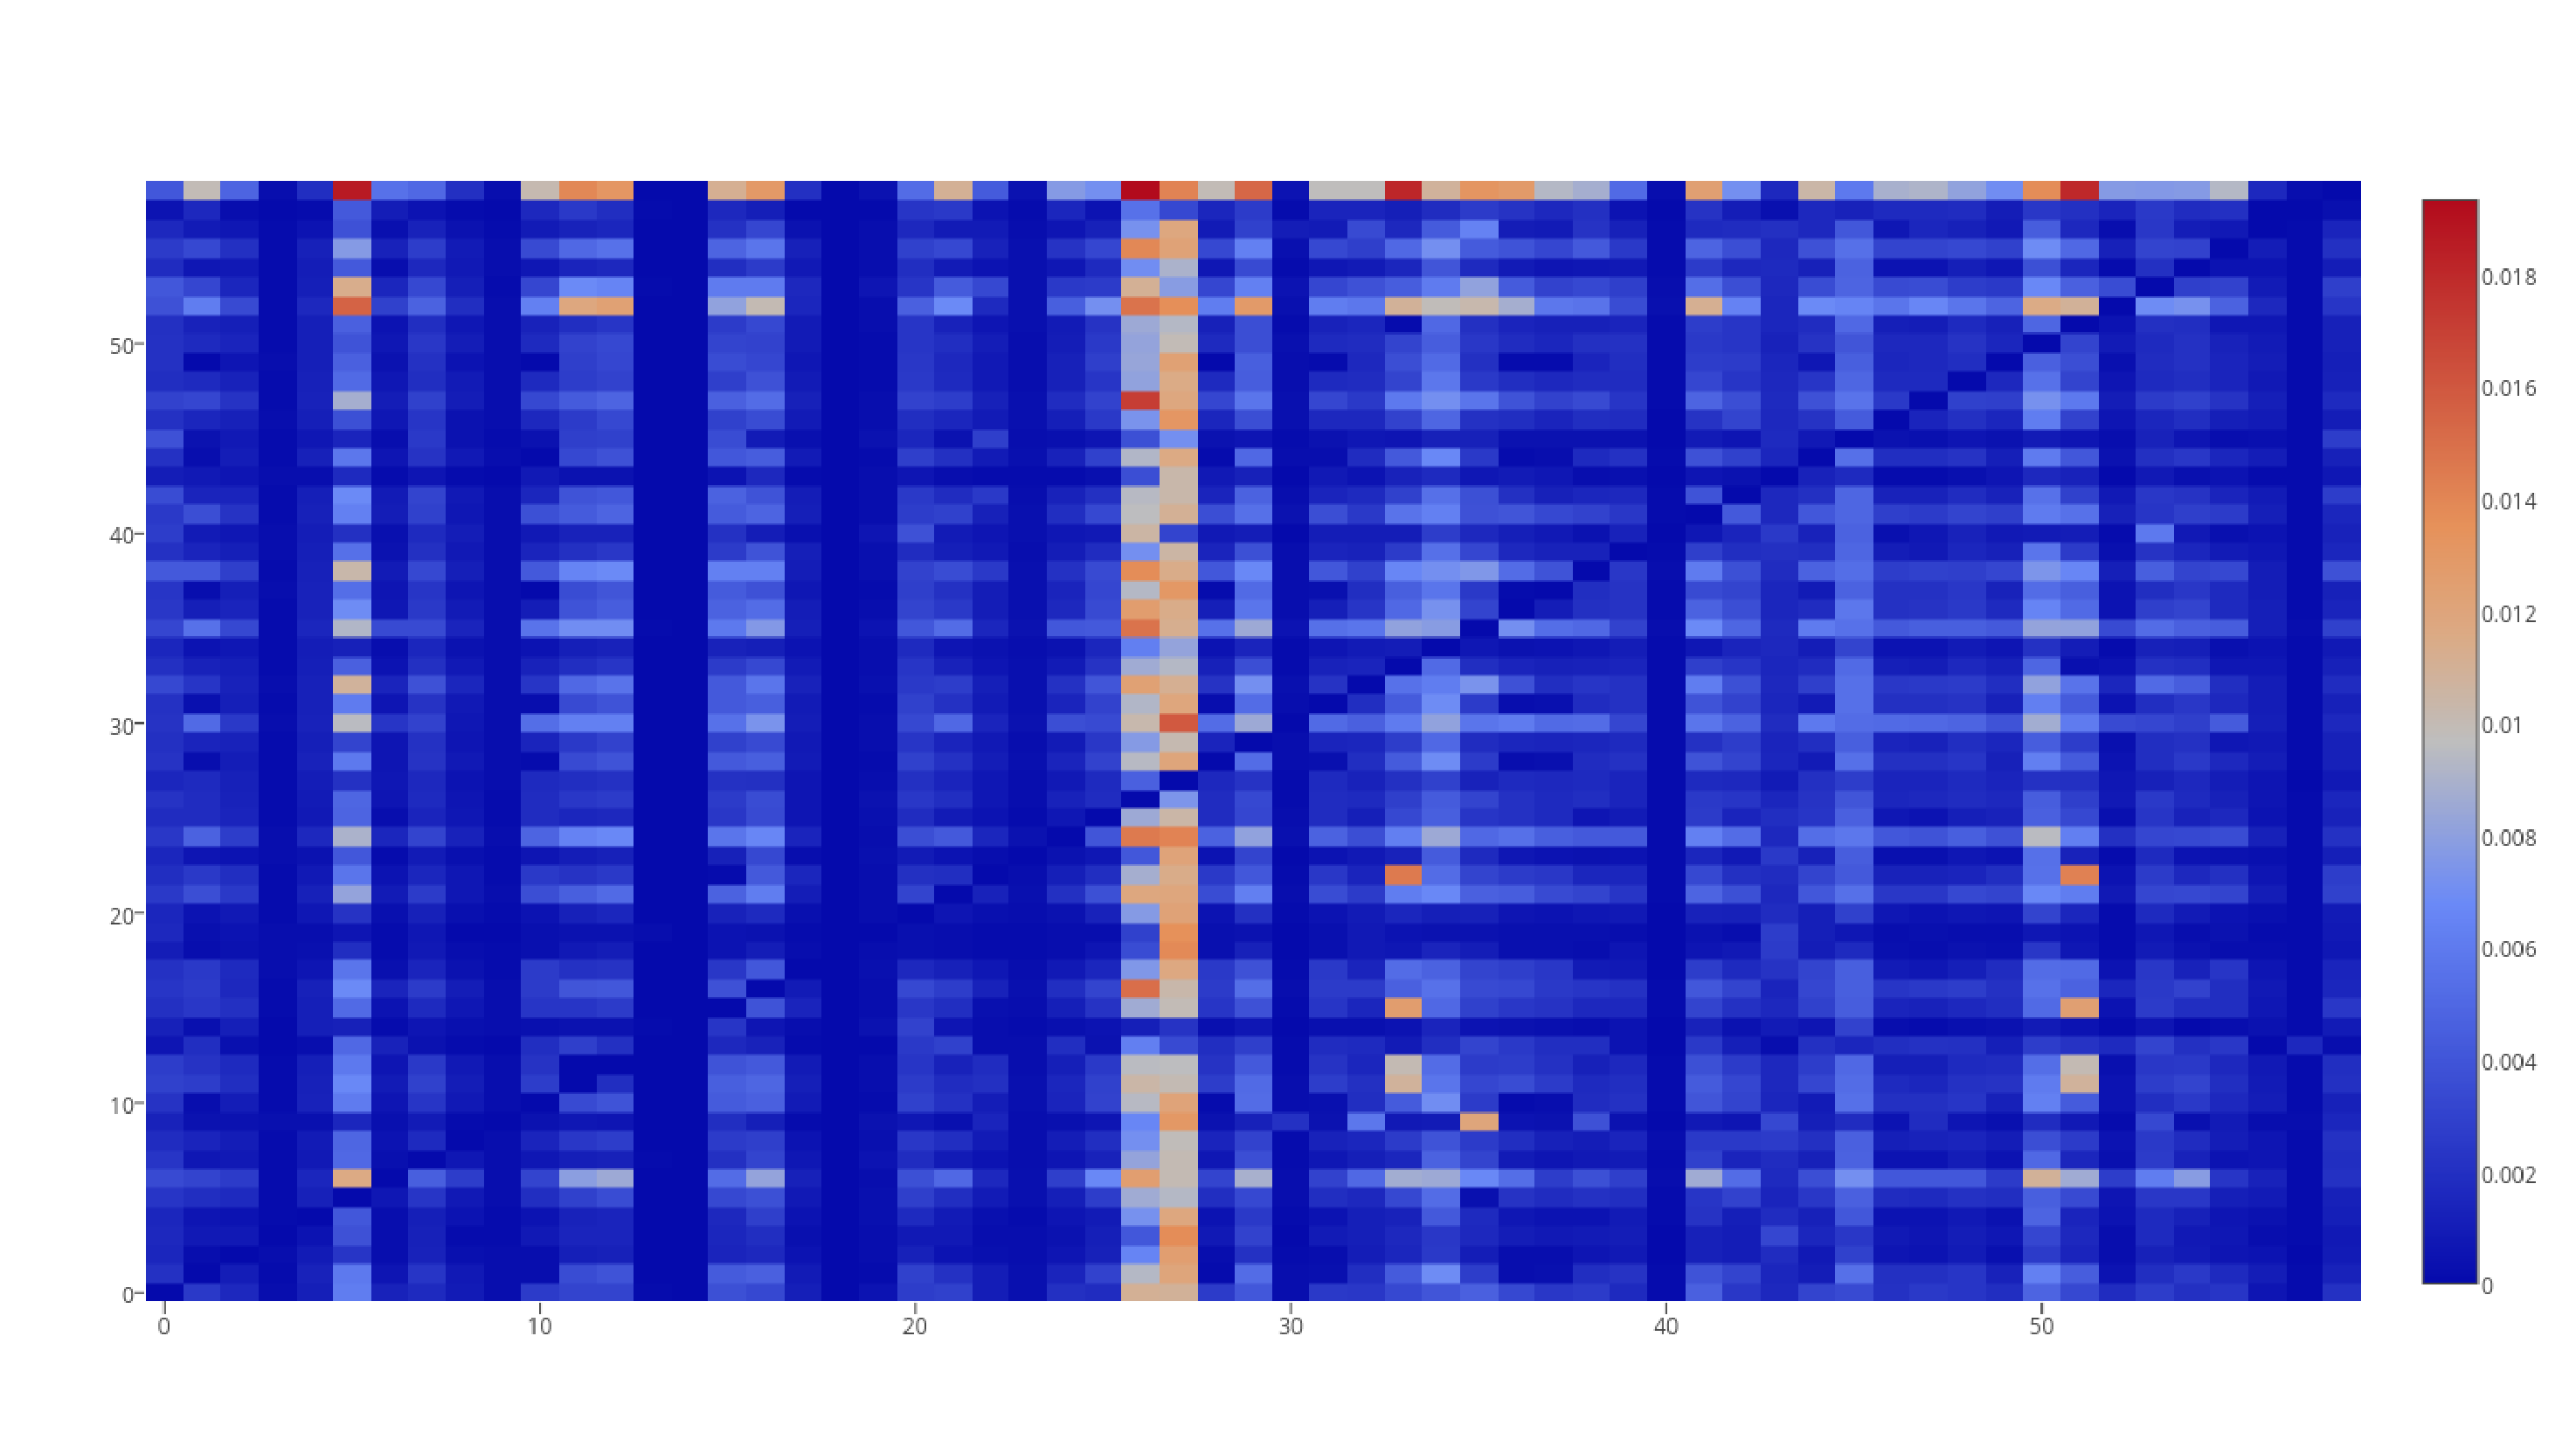
\includegraphics[width=0.24\linewidth]{figure/PC-train}\label{fig:moredata3}} 
\subfloat[]{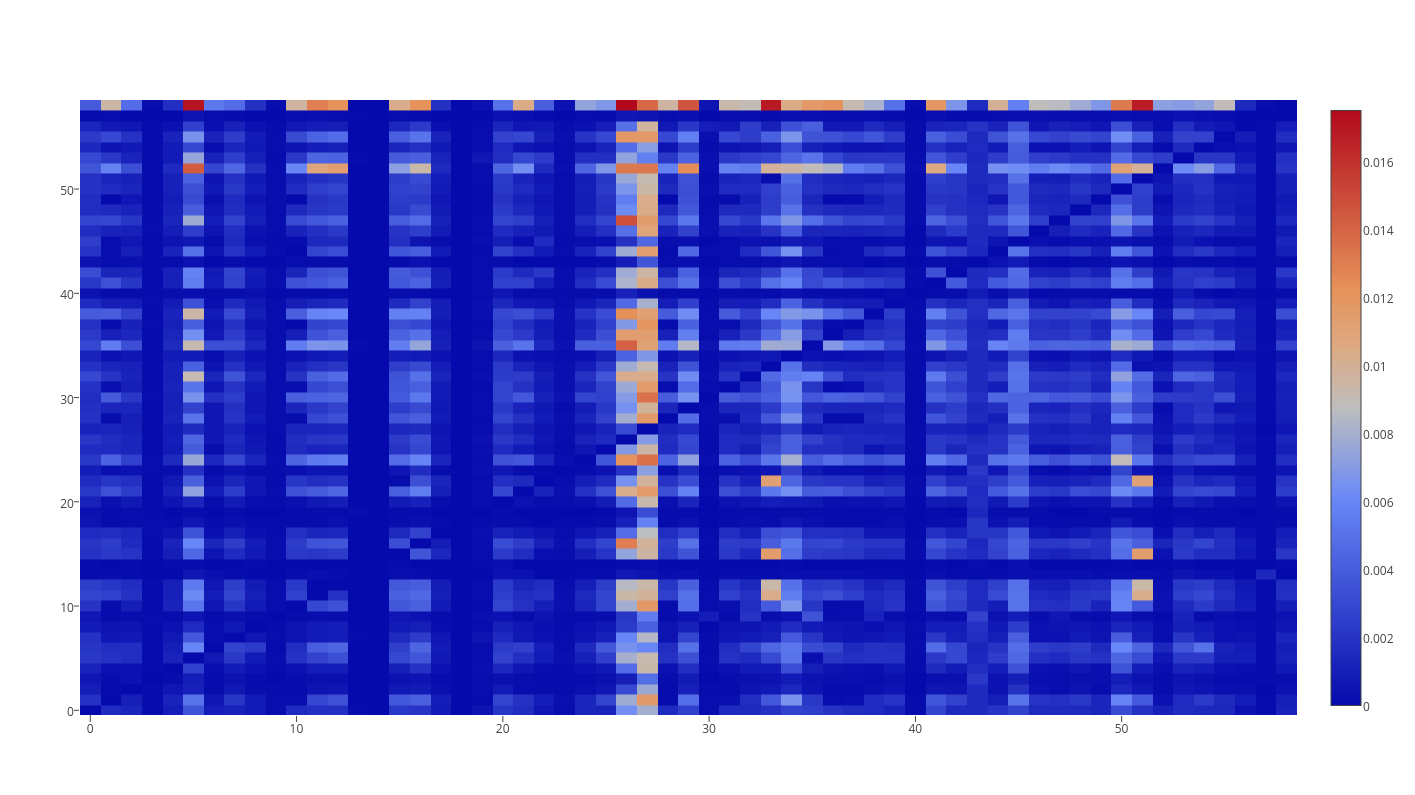
\includegraphics[width=0.24\linewidth]{figure/jaccardPC-train}\label{fig:moredata4}} \\ 
\caption{Potential for 0.5 V bias.} 
\label{fig:EcUND} 
\end{figure*} 


\begin{figure}[t!]
\begin{center}
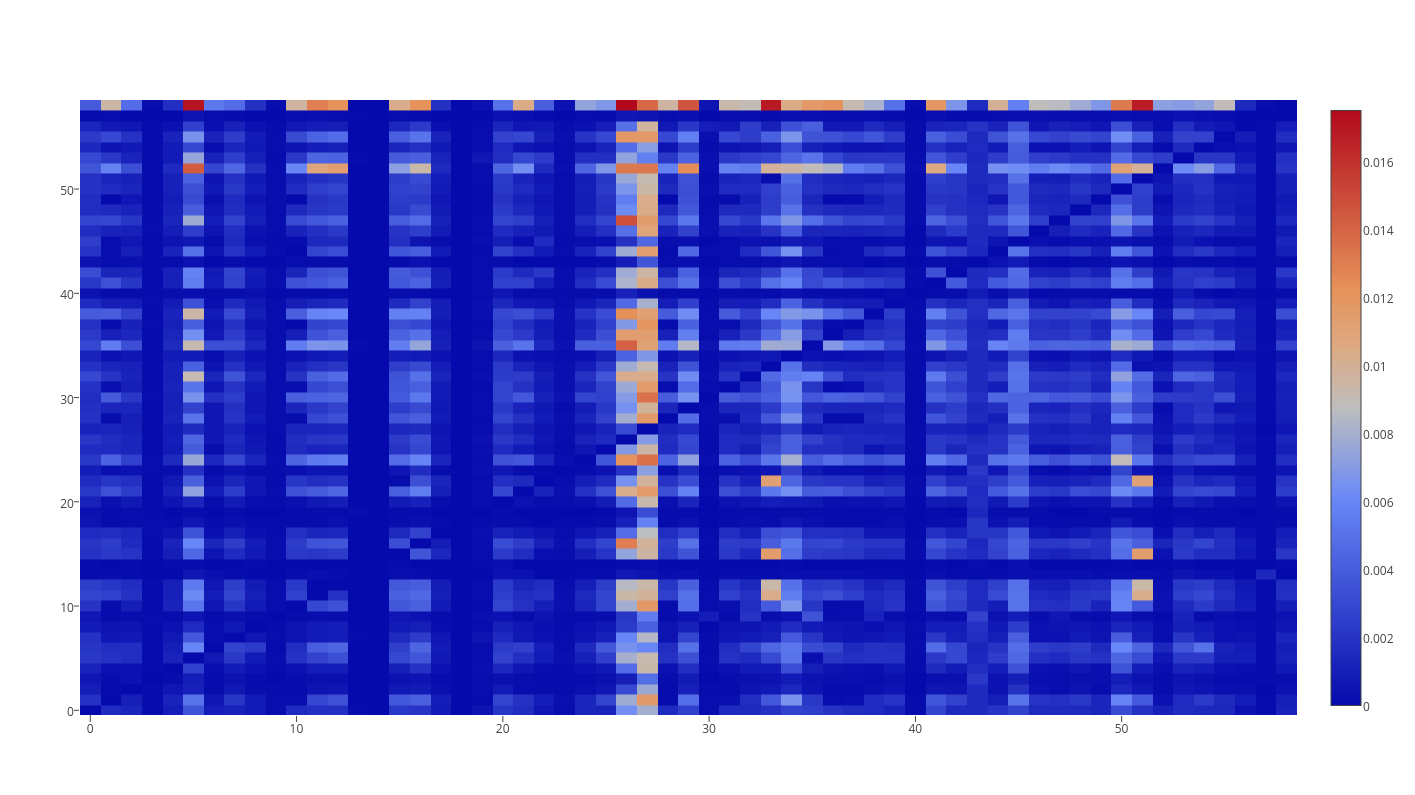
\includegraphics[width=2.5in]{figure/jaccardPC-train}
\mycaption{fig:idreputation}{Test.}
{\footnotesize{(How detection rate changes with the value of source id's reputation. Each reputation is rounded up to nearest 0.05.
Reputation -1 means the source id did not make any submission before. 95\% confidence interval is also drawn 
for each point.)}}
\end{center}
%\vspace{-0.25in}
\end{figure}

From the above analysis, we can see that the influence probability is the key of our anti-virus engine
influence problem.
After knowing the value of the influence probability $p_{u,v}$ between all engine pairs $u$ and $v$,
it is easy to calculate the trustworthiness of all engines.
The problem now boils down to estimating $p_{u,v}$.

To estimate the influence probability between two engines, we propose to use the statistics of actions taken by
an engine on a file and the action propagation between two engines. 
Specifically, we use the {\em happen-after} relationship to
define {\em action propagation}; if an action of an engine is taken after an action of another engine, we say that
this action is propagated.

To assist the definition of action propagation, we first define a few types of submission sets.
We use $A_u$ to represent the set of submissions ever identified by $u$ as malware in its history
and $\bar{A}_u$ to represent the set of submissions that have been labeled as benign and yet not labeled as malware by $u$.
Further, we define the set of actions taken by both $u$ and $v$ as $A_{u\&v}$ 
and the set of actions taken by either $u$ or $v$ as $A_{u|v}$.
Thus, $|A_{u|v}| =   |A_u| + |A_v| - |A_{u\&v}|$.
With these sets defined, we formally
define {\em action propagation} in the following equation 
and use $A_{u2v}$ to represent the set of all the actions that are propagated from $u$ to $v$. 

Action Propagation:
An action $a$ propagated from $u$ to $v$ iff: (i) $\exists$ $(v, \bar{a}, t_i)$ $\in$ $\bar{A}_v$ 
and $(v, a, t_k)$ $\in$ $A_v$, with $t_i < t_k$; (ii) $\exists$ $(u, a, t_j)$ $\in$ $A_u$, with $t_j < t_k$ and $u \neq v$. 


With these definitions, we now present our four proposed static models to estimate $p_{u,v}$.

{\bf Bernoulli distribution} estimates $p_{u,v}$ as the ratio of the number of actions 
propagated from $u$ to $v$ over the total number of actions taken by $u$.

$$p_{u,v} = \frac{|A_{u2v}|}{|A_u|}$$ 

{\bf Jaccard index} estimates 
$p_{u,v}$ as the number of actions propagated from $u$ to $v$ divided by 
the number of actions taken either by $u$ or by $v$.

$$p_{u,v} = \frac{|A_{u2v}|}{|A_{u|v}|}$$ 

On top of the Bernoulli distribution and the Jaccord index,
we add an additional consideration called {\em partial credit}.
When $v$ takes an action $a$, it may be influenced by the combination of all its neighbors $S_v(a)$ 
taking the action $a$ before $v$. %Partial credit takes this intuition. 
To account for this effect, we use partial credit 
and calculate the partial credit for $u$ who takes an action $a$ before $v$ as 

$$credit_{u,v}(a) = \frac{1}{|S_v(a)|}$$

{\bf Bernoulli distribution with partial credit} 
estimates $p_{u,v}$ as the sum of all partial credits taking by $u$ for actions propagated from $u$ to $v$, 
dividing by the number of actions taken by $u$. 

$$p_{u,v} = \frac{\sum\limits_{a \in A_{u2v}}{credit_{u,v}(a)}}{|A_u|}$$

{\bf Jaccard index with partial credit} 
estimates $p_{u,v}$ as the sum of all partial credits taking by $u$ for actions propagated from $u$ to $v$, 
dividing by the number of actions taken either by $u$ or by $v$. 

$$p_{u,v} = \frac{\sum\limits_{a \in A_{u2v}}{credit_{u,v}(a)}}{|A_{u|v}|}$$


%Since $|A_{u|v}|$ is not less than $|A_u|$, 
%$p_{u,v}$ calculated by Jaccard index is not larger than $p_{u,v}$ calculated by Bernoulli distribution. 
%For Bernoulli distribution and Jaccard index, 
%considering partial credit will decrease $p_{u,v}$ calculated by both of them. 


